
\documentclass[border=10pt, 12pt]{standalone}
\usepackage[svgnames]{xcolor}
\usepackage{amsmath}
\usepackage{pgfplots}
\pgfplotsset{compat=newest}
\usepackage[sfdefault]{FiraSans}
\usepackage{FiraMono}
\renewcommand*\familydefault{\sfdefault}
\begin{document}
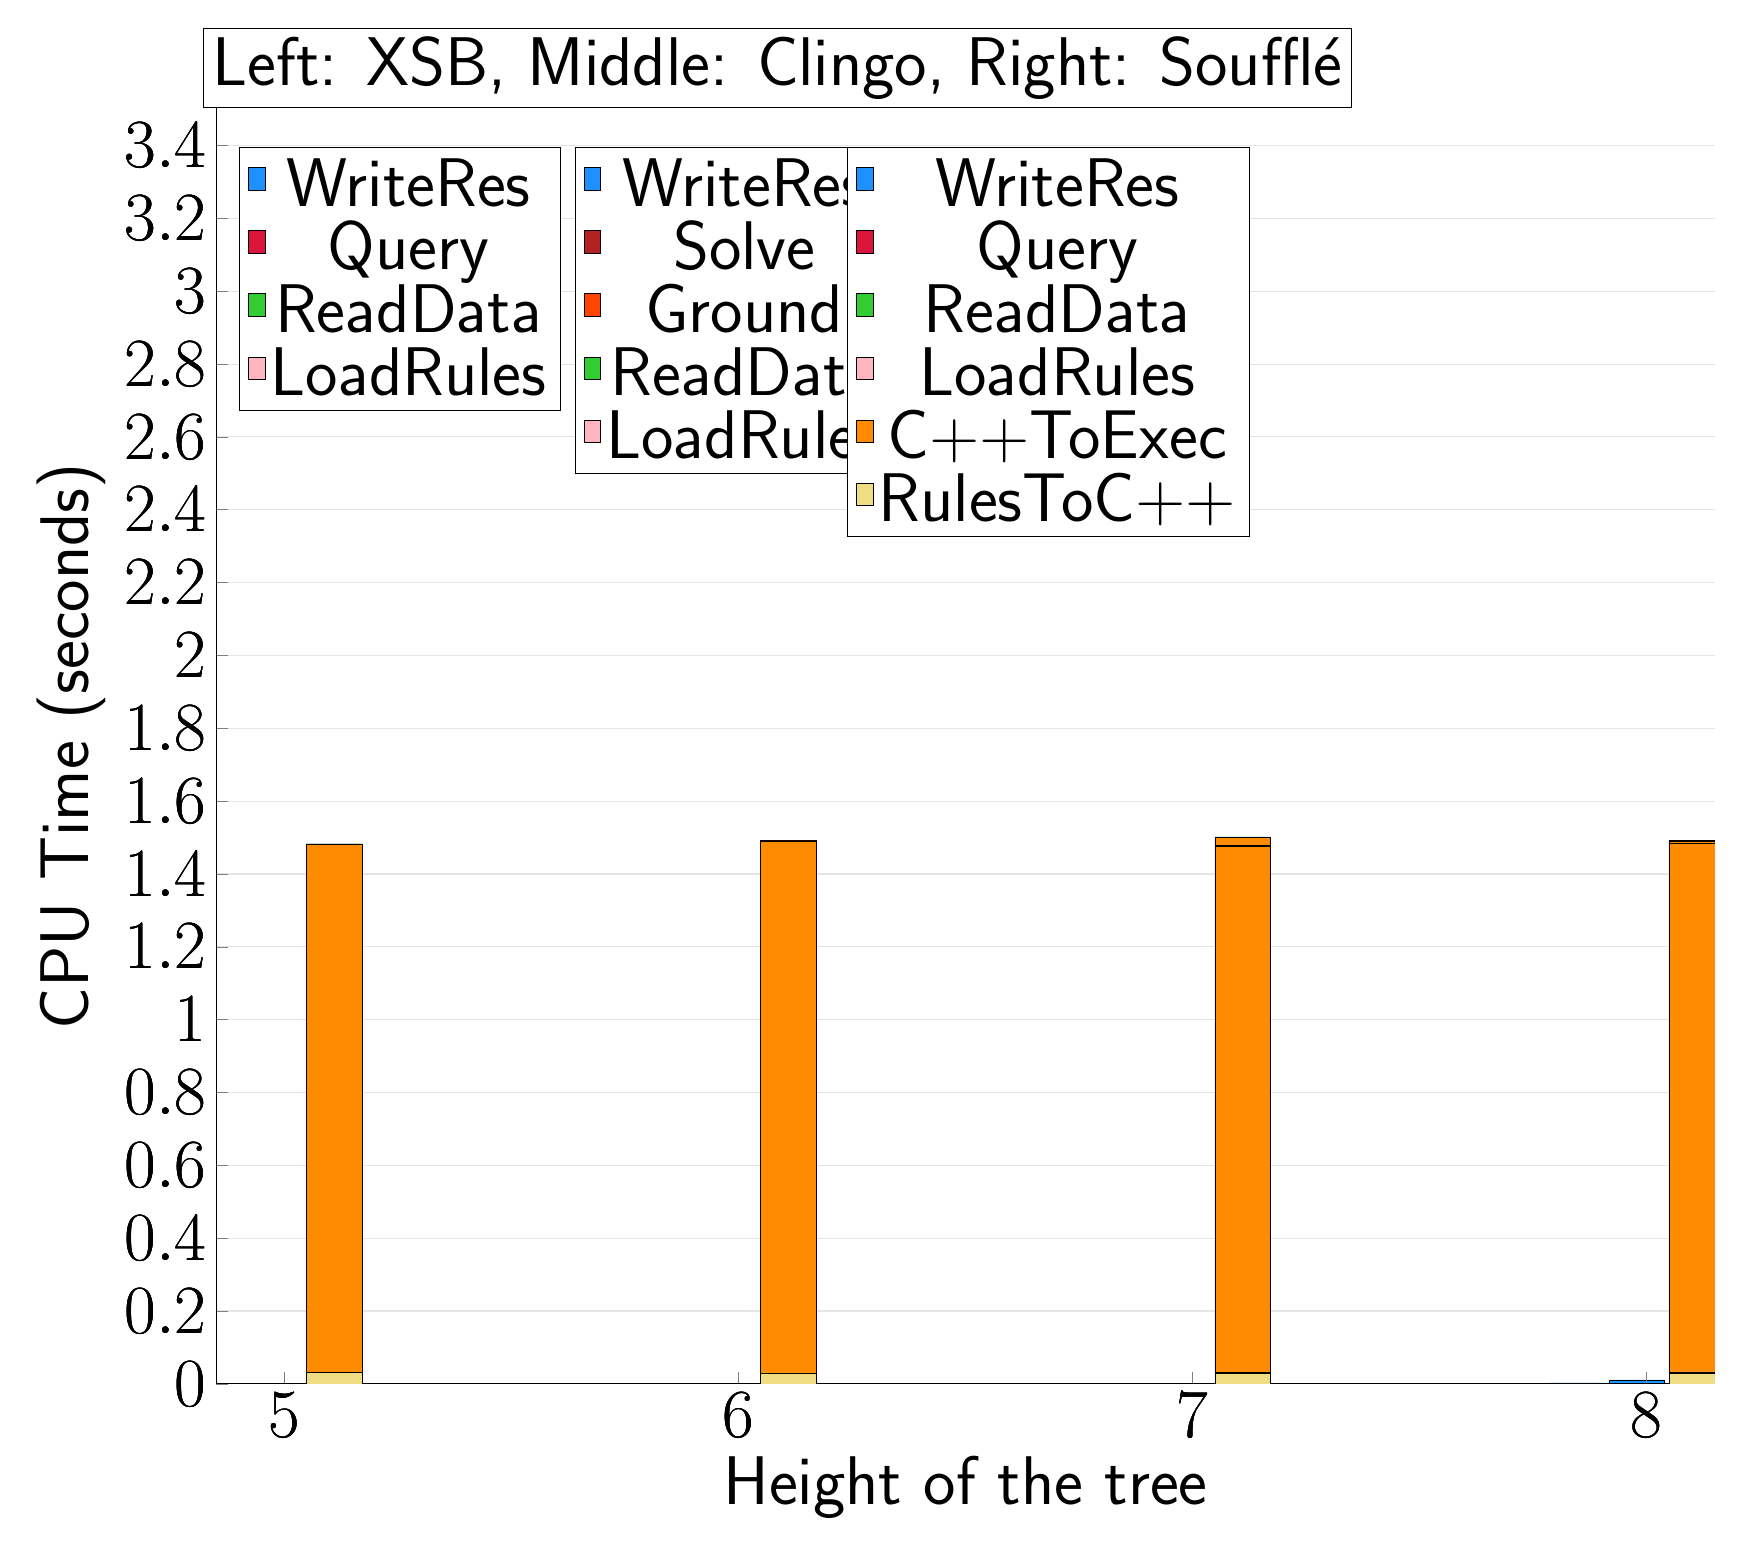
\begin{tikzpicture}
	\begin{axis}[bar shift=-25pt,
			ybar stacked,
			width=1.7\textwidth,
			bar width=0.7cm,
			ymajorgrids, tick align=inside,
			major grid style={draw=gray!20},
			xtick=data,
			ymin=0, ymax=3.5020000000000002,
			axis x line*=bottom,
			axis y line*=left,
			enlarge x limits=0.05,
			legend style={
					at={(0.23, 0.97)},
					anchor=north east,
					legend columns=1,
					font=\Huge,
				},
			ylabel={CPU Time (seconds)},
			xlabel={Height of the tree},
			label style={font=\Huge},
			tick label style={font=\Huge},
		]
		\addlegendimage{fill=DodgerBlue, draw=black, line width=0.2pt}
		\addlegendentry{WriteRes}
		\addlegendimage{fill=Crimson, draw=black, line width=0.2pt}
		\addlegendentry{Query}
		\addlegendimage{fill=LimeGreen, draw=black, line width=0.2pt}
		\addlegendentry{ReadData}
		\addlegendimage{fill=LightPink, draw=black, line width=0.2pt}
		\addlegendentry{LoadRules}
		\addplot +[fill=LightPink, draw=black, line width=0.2pt] coordinates {
				(5, 0.0006007000000000003)
				(6, 0.0005972000000000003)
				(7, 0.0006123000000000003)
				(7, 0.0006026000000000006)
				(7, 0.0006090000000000004)
				(8, 0.0005976000000000003)
				(8, 0.0006092999999999999)
				(8, 0.0006185000000000001)
			};
		\addplot +[fill=LimeGreen, draw=black, line width=0.2pt] coordinates {
				(5, 0.00016139999999999978)
				(6, 0.00018269999999999978)
				(7, 0.00023829999999999972)
				(7, 0.0002412999999999998)
				(7, 0.00024109999999999982)
				(8, 0.0003510000000000001)
				(8, 0.0003514000000000001)
				(8, 0.00035729999999999974)
			};
		\addplot +[fill=Crimson, draw=black, line width=0.2pt] coordinates {
				(5, 2.2000000000000155e-05)
				(6, 3.6000000000000096e-05)
				(7, 6.960000000000042e-05)
				(7, 6.920000000000019e-05)
				(7, 6.950000000000014e-05)
				(8, 0.00014489999999999992)
				(8, 0.0001466)
				(8, 0.0001489000000000004)
			};
		\addplot +[fill=DodgerBlue, draw=black, line width=0.2pt] coordinates {
				(5, 0.0001561000000000001)
				(6, 0.00030479999999999944)
				(7, 0.0006472999999999997)
				(7, 0.0006433999999999997)
				(7, 0.0006484)
				(8, 0.001446)
				(8, 0.001462)
				(8, 0.0014440999999999996)
			};
	\end{axis}

	\begin{axis}[bar shift=-3.7pt,
			ybar stacked,
			width=1.7\textwidth,
			bar width=0.7cm,
			ymajorgrids, tick align=inside,
			major grid style={draw=none},
			xtick=data,
			ymin=0, ymax=3.5020000000000002,
			axis x line*=none,
			axis y line*=none,
			enlarge x limits=0.05,
			legend style={
					at={(0.454, 0.97)},
					anchor=north east,
					legend columns=1,
					font=\Huge,
				},
			label style={font=\Huge},
			tick label style={font=\Huge},
		]
		\addlegendimage{fill=DodgerBlue, draw=black, line width=0.2pt}
		\addlegendentry{WriteRes}
		\addlegendimage{fill=FireBrick, draw=black, line width=0.2pt}
		\addlegendentry{Solve}
		\addlegendimage{fill=OrangeRed, draw=black, line width=0.2pt}
		\addlegendentry{Ground}
		\addlegendimage{fill=LimeGreen, draw=black, line width=0.2pt}
		\addlegendentry{ReadData}
		\addlegendimage{fill=LightPink, draw=black, line width=0.2pt}
		\addlegendentry{LoadRules}
		\addplot +[fill=LightPink, draw=black, line width=0.2pt] coordinates {
				(5, 0.0)
				(6, 0.0)
				(7, 0.0)
				(7, 0.0)
				(7, 0.0)
				(8, 0.0)
				(8, 0.0)
				(8, 0.0)
			};
		\addplot +[fill=LimeGreen, draw=black, line width=0.2pt] coordinates {
				(5, 0.0)
				(6, 0.0)
				(7, 0.0)
				(7, 0.0)
				(7, 0.0)
				(8, 0.0)
				(8, 0.0)
				(8, 0.0)
			};
		\addplot +[fill=OrangeRed, draw=black, line width=0.2pt] coordinates {
				(5, 0.0)
				(6, 0.0)
				(7, 0.0)
				(7, 0.0)
				(7, 0.0009999999999999998)
				(8, 0.0)
				(8, 0.0)
				(8, 0.0)
			};
		\addplot +[fill=FireBrick, draw=black, line width=0.2pt] coordinates {
				(5, 0.0)
				(6, 0.0)
				(7, 0.0)
				(7, 0.0)
				(7, 0.0)
				(8, 0.0009999999999999998)
				(8, 0.0)
				(8, 0.0)
			};
		\addplot +[fill=DodgerBlue, draw=black, line width=0.2pt] coordinates {
				(5, 0.0)
				(6, 0.0)
				(7, 0.0)
				(7, 0.0)
				(7, 0.0)
				(8, 0.009999999999999997)
				(8, 0.009999999999999997)
				(8, 0.009999999999999997)
			};
	\end{axis}

	\begin{axis}[bar shift=18pt,
			ybar stacked,
			width=1.7\textwidth,
			bar width=0.7cm,
			ymajorgrids, tick align=inside,
			major grid style={draw=none},
			xtick=data,
			ymin=0, ymax=3.5020000000000002,
			axis x line*=none,
			axis y line*=none,
			enlarge x limits=0.05,
			legend style={
					at={(0.69, 0.97)},
					anchor=north east,
					legend columns=1,
					font=\Huge,
				},
			label style={font=\Huge},
			tick label style={font=\Huge},
		]
		\addlegendimage{fill=DodgerBlue, draw=black, line width=0.2pt}
		\addlegendentry{WriteRes}
		\addlegendimage{fill=Crimson, draw=black, line width=0.2pt}
		\addlegendentry{Query}
		\addlegendimage{fill=LimeGreen, draw=black, line width=0.2pt}
		\addlegendentry{ReadData}
		\addlegendimage{fill=LightPink, draw=black, line width=0.2pt}
		\addlegendentry{LoadRules}
		\addlegendimage{fill=DarkOrange, draw=black, line width=0.2pt}
		\addlegendentry{C++ToExec}
		\addlegendimage{fill=LightGoldenrod, draw=black, line width=0.2pt}
		\addlegendentry{RulesToC++}
		\addplot +[fill=LightGoldenrod, draw=black, line width=0.2pt] coordinates {
				(5, 0.031999999999999994)
				(6, 0.030000000000000006)
				(7, 0.030000000000000006)
				(7, 0.030000000000000006)
				(7, 0.031000000000000007)
				(8, 0.030000000000000006)
				(8, 0.030000000000000006)
				(8, 0.032999999999999995)
			};
		\addplot +[fill=DarkOrange, draw=black, line width=0.2pt] coordinates {
				(5, 1.4499999999999997)
				(6, 1.4600000000000002)
				(7, 1.4449999999999998)
				(7, 1.4479999999999997)
				(7, 1.4689999999999999)
				(8, 1.454)
				(8, 1.459)
				(8, 1.4499999999999997)
			};
		\addplot +[fill=LightPink, draw=black, line width=0.2pt] coordinates {
				(5, 0.0)
				(6, 0.0)
				(7, 0.0)
				(7, 3.12e-05)
				(7, 0.0)
				(8, 0.0)
				(8, 1.01e-05)
				(8, 0.0)
			};
		\addplot +[fill=LimeGreen, draw=black, line width=0.2pt] coordinates {
				(5, 0.0003510000000000001)
				(6, 0.0004326)
				(7, 0.0005727000000000001)
				(7, 0.0005906)
				(7, 0.0005552)
				(8, 0.0008234999999999999)
				(8, 0.0008766000000000002)
				(8, 0.0008435)
			};
		\addplot +[fill=Crimson, draw=black, line width=0.2pt] coordinates {
				(5, 0.00011040000000000001)
				(6, 0.0003412)
				(7, 0.000821)
				(7, 0.0008640999999999999)
				(7, 0.0007863999999999999)
				(8, 0.0019447999999999996)
				(8, 0.0020185)
				(8, 0.0019312999999999997)
			};
		\addplot +[fill=DodgerBlue, draw=black, line width=0.2pt] coordinates {
				(5, 0.0002695)
				(6, 0.00032779999999999994)
				(7, 0.00048110000000000004)
				(7, 0.0005166)
				(7, 0.00045460000000000005)
				(8, 0.0009165)
				(8, 0.000911)
				(8, 0.0009096)
			};
	\end{axis}


	\node[anchor=south, draw, fill=white] at (rel axis cs:0.42,1) {\Huge Left: XSB, Middle: Clingo, Right: Soufflé};
\end{tikzpicture}
\end{document}
